\documentclass[12pt, dvipdfmx]{beamer}
\let\Tiny=\tiny
\usepackage{graphicx}
\usetheme{metropolis}
\usefonttheme[onlymath]{serif}
\usepackage[uplatex, deluxe, expert]{otf}
\renewcommand{\kanjifamilydefault}{\gtdefault}
\usepackage{textcomp}
\usepackage{type1cm}
\usepackage{listings}
\usepackage{color}
\usepackage{pxjahyper}

\title{引き継ぎ資料 Vol.2}
\subtitle{Pythonに関する諸々}
\date{2016/06/16}
\author{}
\institute{}
\begin{document}
\maketitle
\begin{frame}{目次}
  \setbeamertemplate{section in toc}[sections numbered]
  \tableofcontents[hideallsubsections]
\end{frame}
\begin{frame}{注意事項}
    基本的文法はについては\alert{省略}します

    適宜質問してください
\end{frame}
\begin{frame}{コードについて}
    \begin{itemize}
        \item 今日のコードとプレゼンは\url{https://github.com/xi-xi/takeover_document}

        \item \alert{何かあればIssuesに書いてください}
        \item 公開レポジトリなので実名公開しないように!
    \end{itemize}
\end{frame}

\section{Pythonとは?}
\begin{frame}
    \begin{figure}[htbp]
        \centering
        
\includegraphics[width=0.8\textwidth]{img/pythonlogo.pdf}
    \end{figure}
    \begin{quote}
        Python is a programming language that lets you work quickly and integrate systems more effectively
    \end{quote}
    \begin{flushright}
        (\url{https://www.python.org})
    \end{flushright}
\end{frame}
\begin{frame}{Pythonとは?}
    近年人気なスクリプト言語

    \begin{block}<2->{人気なジャンル}
        \begin{itemize}
            \item 機械学習
            \item データ解析...
        \end{itemize}
    \end{block}

    \begin{block}<3->{採用実績}
        \begin{itemize}
            \item Google
            \item Dropbox...
        \end{itemize}
    \end{block}
\end{frame}
\begin{frame}{Pythonのいいところ・よくないところ}
    \begin{alertblock}{Pros}
        \begin{itemize}
            \item 標準ライブラリが強力
            \item 標準以外のライブラリも充実
            \item 書くのがとっても楽
            \item 同じ意味を書くために1つのやり方
        \end{itemize}
    \end{alertblock}
    \begin{block}{Cons}
        \begin{itemize}
            \item 遅い
            \item (個人的には)型に厳密であってほしい    
        \end{itemize}
    \end{block}
\end{frame}

\section{Pythonの環境構築}
\begin{frame}{Python環境を整えよう}
    MacにはPythonがデフォルト搭載

    デフォルトのPythonを使えばいい?

    \pause
    \textbf{\alert{よくない!}}
\end{frame}
\begin{frame}{デフォルトのPythonを使うと...}
    \begin{itemize}
        \item PythonのバージョンがOS依存
        \begin{itemize}
            \item Macのデフォルトは2.7
            \item イマドキのいけてる人は3.5
        \end{itemize}
        \item OSのアップデートで(もしかしたら)環境が破壊
        \item 自分で入れたライブラリがOSと競合する可能性
        \item 気軽に環境のリセットとかできない
    \end{itemize}
\end{frame}
\begin{frame}{じゃあどうするの?}
    \begin{center}
        {\Huge pyenv + Anaconda}
    \end{center}
\end{frame}
\defverbatim[colored]\installpyenv{%
\begin{lstlisting}[basicstyle=\small\ttfamily]
$ pyenv install 3.5.1
\end{lstlisting}
}
\defverbatim[colored]\usepyenv{%
\begin{lstlisting}[basicstyle=\small\ttfamily]
$ pyenv local 3.5.1
\end{lstlisting}
}
\begin{frame}{pyenvとは}
    \begin{itemize}
        \item 複数のPythonバージョンを取り替えられる
        \item Homebrewを使ってインストール可
    \end{itemize}
    \begin{exampleblock}{超簡単な使い方}
        python 3.5.1をインストール
        \installpyenv

        カレント以下では3.5.1を使用
        \usepyenv
    \end{exampleblock}
\end{frame}
\begin{frame}
    \begin{figure}[htbp]
        \centering
        
\includegraphics[width=0.8\textwidth]{img/anacondalogo.pdf}
    \end{figure}
    \begin{quote}
        Leading Open Data Science Platform Powered by Python
    \end{quote}
    \begin{flushright}
        (\url{https://www.continuum.io/why-anaconda})
    \end{flushright}
\end{frame}
\begin{frame}{Anacondaとは}
    \begin{itemize}
        \item 様々なライブラリをデフォルトで搭載
        \begin{itemize}
            \item numpy, matplotlib, scipy…
        \end{itemize}
        \item ライブラリ管理コマンドのcondaが付属
        \begin{itemize}
            \item pipとは別物
            \begin{itemize}
                \item pipはソースをDLしてコンパイル
                \item condaはバイナリをインストール
            \end{itemize}
        \end{itemize}
        \item<2|alert@2> とっても楽に環境構築が可能
    \end{itemize}
\end{frame}
\defverbatim[colored]\installanaconda{%
\begin{lstlisting}[basicstyle=\small\ttfamily]
$ pyenv install anaconda3-4.0.0
\end{lstlisting}
}
\defverbatim[colored]\useanaconda{%
\begin{lstlisting}[basicstyle=\small\ttfamily]
$ pyenv local anaconda3-4.0.0
\end{lstlisting}
}
\begin{frame}{pyenv + Anacondaによる環境構築}
    \begin{block}{Mac}
        \begin{enumerate}
            \item Anacondaのインストール(時間大)
            \installanaconda
            \item カレント以下で使用を宣言
            \useanaconda
        \end{enumerate}
    \end{block}
    \begin{exampleblock}{(参考)Windows}
        Anacondaインストーラを実行
    \end{exampleblock}
\end{frame}

\section{Pythonで便利な構文}
\begin{frame}{話す内容}
    \begin{itemize}
        \item ワンライナー
        \item 特殊メソッド
    \end{itemize}
\end{frame}
\defverbatim[colored]\onelinear{%
\begin{lstlisting}[language=Python,basicstyle=\ttfamily,numbers=left, keywordstyle=\color{blue}\ttfamily, stringstyle=\color{red}]
normal = []
for i in range(10):
    normal.append(i)
one = [i for i in range(10)]
\end{lstlisting}
}
\begin{frame}{ワンライナー}
    なんでも一行でかける素敵な構文

    \onelinear

    ここでnormalとoneは同じ

    \alert{使い過ぎると読みにくくなるので注意}
\end{frame}
\defverbatim[colored]\wronglinear{%
\begin{lstlisting}[language=Python,basicstyle=\ttfamily,numbers=left, keywordstyle=\color{blue}\ttfamily, stringstyle=\color{red}]
def load_csv(filename):
    with open(filename) as f:
        return [
            [cell for cell in row]
            for row in csv.reader(f)
        ]
\end{lstlisting}
}
\begin{frame}{やっちゃったワンライナー}
    \wronglinear
\end{frame}
\begin{frame}{特殊メソッド}
    特定の構文を使う際にPythonによって呼び出される関数

    \_\_init\_\_,\_\_call\_\_,\_\_str\_\_など様々
\end{frame}
\defverbatim[colored]\specialfunc{%
\begin{lstlisting}[language=Python,basicstyle=\scriptsize\ttfamily,numbers=left, keywordstyle=\color{blue}\ttfamily, stringstyle=\color{red}, commentstyle=\color{green}]
class QuadraticFunction:
    def __init__(self, a, b, c):
        self.a = a
        self.b = b
        self.c = c

    def __call__(self, x):
        return self.a * x ** 2 + self.b * x + self.c

    def __str__(self):
        return "{}x^2+{}x+{}".format(self.a, self.b, self.c)
def main():
    fx = QuadraticFunction(1, 2, 1) #call fx.__init__(1,2,1)
    print(str(fx)) #call fx.__str__()
    for x in range(10):
        print(fx(x)) #call fx.__call__(x)
\end{lstlisting}
}
\begin{frame}{例}
    \specialfunc
\end{frame}
\begin{frame}{特殊メソッド}
    特定の構文を使う際にPythonによって呼び出される関数

    \_\_init\_\_,\_\_call\_\_,\_\_str\_\_など様々

    うまく使うと関数のようなクラスインスタンスも作成可能
\end{frame}

\section{Pythonプログラムを良くするちょっとしたこと}
\begin{frame}{心得とか}
    \begin{itemize}
        \item エディタにはPEPチェックを導入
        \item Google Python Style Guideを参考\\
            {\small\url{https://google.github.io/styleguide/pyguide.html}}
        \begin{itemize}
            \item 使うべき文法
            \item 使うべきでない文法
            \item 命名規則
            \item コメントの書き方
        \end{itemize}
    \end{itemize}
\end{frame}
\begin{frame}{覚えておくと便利な関数}
    \begin{itemize}
        \item zip
        \item enumerate
    \end{itemize}
\end{frame}
\defverbatim[colored]\zipsample{%
\begin{lstlisting}[language=Python,basicstyle=\ttfamily,numbers=left, keywordstyle=\color{blue}\ttfamily, stringstyle=\color{red}]
def main():
    a_list = [1, 2, 3]
    b_list = [4, 5, 6]
    for a, b in zip(a_list, b_list):
        print(a, b)
\end{lstlisting}
}
\begin{frame}{zip}
    2つのリストを同時にループ
    \zipsample
\end{frame}
\defverbatim[colored]\enumsample{%
\begin{lstlisting}[language=Python,basicstyle=\ttfamily,numbers=left, keywordstyle=\color{blue}\ttfamily, stringstyle=\color{red}]
def main():
    a_list = ["a", "b", "c"]
    for i, a in enumerate(a_list):
        print(i, a)
\end{lstlisting}
}
\begin{frame}{enumerate}
    indexと要素を同時に取得
    \enumsample
\end{frame}

\section{データのロード}
\begin{frame}{データのロード}
    Pythonは一般的なファイル形式をサポート
    \begin{itemize}
        \item \alert<2>{csv}
        \item \alert<2>{json}
        \item xml
        \item html
        \item gzip...
    \end{itemize}
\end{frame}
\begin{frame}{csvファイルとは?}
    \begin{itemize}
        \item カンマで句切られた値が並ぶテキスト
        \item 要は表
        \item Excelなどでも読み書き可能
    \end{itemize}
    \begin{columns}
        \begin{column}{0.5\textwidth}
            \begin{table}[h]
                \begin{tabular}{|l|}
                    \hline
                    Name,Height,Weight\\
                    Hoge Taro,155,40\\
                    Fuga Hanako,165,50\\
                    Hoga Ta,175,60\\\hline
                \end{tabular}
            \end{table}
        \end{column}
        \begin{column}{0.5\textwidth}
            \begin{figure}[h]
                \centering
                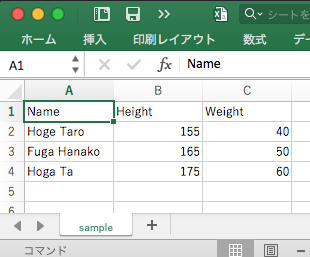
\includegraphics[width=4cm]{img/excel_csv.png}
            \end{figure}
        \end{column}
    \end{columns}
\end{frame}
\defverbatim[colored]\loadcsvpython{%
\begin{lstlisting}[language=Python,basicstyle=\tiny\ttfamily,numbers=left, keywordstyle=\color{blue}\ttfamily, stringstyle=\color{red}]
import sys
import csv


def main(filename):
    with open(filename) as f:
        for row in csv.reader(f):
            for cell in row:
                print(cell)

if __name__ == '__main__':
    main(sys.argv[1])
\end{lstlisting}
}
\begin{frame}{Pythonによるcsvの読み込み}
    \begin{columns}[t]
        \begin{column}{0.5\textwidth}
            \begin{block}{コード}
                \loadcsvpython
            \end{block}
        \end{column}
        \begin{column}{0.5\textwidth}
            \begin{block}{結果}
                \begin{figure}[h]
                    \centering
                    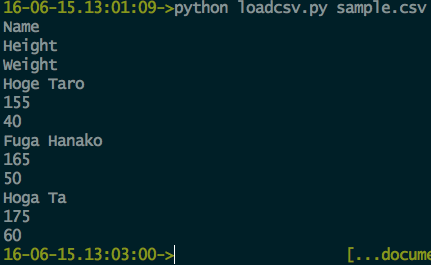
\includegraphics[width=4.2cm]{img/load_csv_result.png}
                \end{figure}
            \end{block}
        \end{column}
    \end{columns}
\end{frame}
\begin{frame}{標準以外のライブラリの場合}
    pandasを使えば一行

    調べればすぐわかるので省略
\end{frame}
\defverbatim[colored]\loadcsvcpp{%
\begin{lstlisting}[language=C++,basicstyle=\tiny\ttfamily,numbers=left, keywordstyle=\color{blue}\ttfamily, stringstyle=\color{red}]
#include <iostream>
#include <fstream>
#include <string>
#include <sstream>

int main(int argc, char** argv){
    std::string filename = argv[1];
    std::ifstream f(filename);
    std::string row;
    while(std::getline(f, row)){
        std::istringstream ss(row);
        std::string cell;
        while(std::getline(ss, cell, ',')){
            std::cout << cell << std::endl;
        }
    }
}
\end{lstlisting}
}
\begin{frame}{余談: C++によるcsvの読み込み}
    \loadcsvcpp

    \pause
    \alert{Pythonの方がはるかに楽}
\end{frame}
\begin{frame}{課題: csvファイルの読み込み\&プロット}
    \begin{itemize}
        \item dummy\_data.csvの中身をプロットしよう
        \item 1行目がx,2行目がy
    \end{itemize}
    \begin{exampleblock}{ヒント}
        \begin{itemize}
            \item プロットはmatplotlibのscatter関数
            \item scatter関数: scatter(x,y)
            \item scatter関数にはnumpy.array型を渡すとプロット
        \end{itemize}    
    \end{exampleblock}
\end{frame}
\begin{frame}{jsonファイルとは?}
    \begin{columns}[t]
        \begin{column}{0.6\textwidth}
            \begin{itemize}
                \item JavaScript Object Notation
                \item Pythonのようなデータ構造
                \begin{itemize}
                    \item List
                    \item Dictionary
                \end{itemize}
                \item Web界隈で広く使われる形式
            \end{itemize}
        \end{column}
        \begin{column}{0.4\textwidth}
            \begin{block}{sample.json}
            {\tiny
            \{\\
            \hspace{4em}    "Hoge Taro": \{\\
            \hspace{8em}        "Height": 155,\\
            \hspace{8em}        "Weigth": 40\\
            \hspace{4em}    \},\\
            \hspace{4em}    "Fuga Hanako": \{\\
            \hspace{8em}        "Height": 165,\\
            \hspace{8em}        "Weigth": 50\\
            \hspace{4em}    \},\\
            \hspace{4em}    "Hoga Ta": \{\\
            \hspace{8em}        "Height": 175,\\
            \hspace{8em}        "Weigth": 50\\
            \hspace{4em}    \}\\
            \}\\
            }
            \end{block}
        \end{column}
    \end{columns}
\end{frame}
\defverbatim[colored]\loadjsonpython{%
\begin{lstlisting}[language=Python,basicstyle=\tiny\ttfamily,numbers=left, keywordstyle=\color{blue}\ttfamily, stringstyle=\color{red}]
import sys
import json

def main(filename):
    with open(filename) as f:
        data = json.load(f)
        print(data)

if __name__ == '__main__':
    main(sys.argv[1])
\end{lstlisting}
}
\begin{frame}{Pythonによるjsonの読み込み}
    \begin{columns}[t]
        \begin{column}{0.5\textwidth}
            \begin{block}{コード}
                \loadjsonpython
            \end{block}
        \end{column}
        \begin{column}{0.5\textwidth}
            \begin{block}{結果}
                \begin{figure}[h]
                    \centering
                    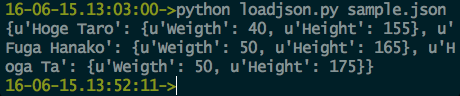
\includegraphics[width=4.2cm]{img/load_json_result.png}
                \end{figure}
            \end{block}
        \end{column}
    \end{columns}
\end{frame}
\begin{frame}[standout]
  Questions?
\end{frame}
\end{document}
